\documentclass{article}
\usepackage[english]{babel}
\usepackage[utf8]{inputenc}
\usepackage{fancyhdr}
\usepackage{geometry}
\usepackage{enumitem}
\usepackage{amsmath}
\usepackage{graphicx}
\usepackage{tcolorbox}
\usepackage{amssymb}
\usepackage[thinc]{esdiff}
\usepackage{float}
\usepackage{caption}

%%%%%%%%%%%%%%%%%%%%%%%%%%%%%%%%%%%%%%%%%%%%%%%%%%%%%%%%%%%%%%%%%%%%%%%%%%%%%%%%%%%%%%%%%%%% DOCUMENT SETUP


\geometry{letterpaper, portrait, margin=1in}
\graphicspath{ {images/} }
\pagestyle{fancy}
\fancyhf{}
\lhead{Keerthik Muruganandam}
\rhead{Yadavalli Written Work 8}


\begin{document}

\begin{enumerate}[label=\textbf{(8.\arabic*)}]

%%%%%%%%%%%%%%%%%%%%%%%%%%%%%%%%%%%%%%%%%%%%%%%%%%%%%%%%%%%%%%%%%%%%%%%%%%%%%%%%%%%%%%%%%%%% 8.1 PROBLEM


\item Set up integrals for the volume of each of the solids below. The base of each solid is the region bounded by $y=1-x$ and $y=x^2-1$. The cross sections perpendicular to the $x$-axis are describe below
\begin{figure}[H]
    \centering
    \begin{minipage}{0.33\textwidth}
        \centering
        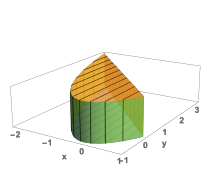
\includegraphics[scale=.5]{rect} % first figure itself
        \caption*{(a) Rectangles of height 2}
    \end{minipage}\hfill
    \begin{minipage}{0.33\textwidth}
        \centering
        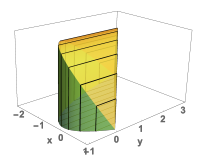
\includegraphics[scale=.5]{sqr} % second figure itself
        \caption*{(b) Squares}
    \end{minipage}
        \begin{minipage}{0.33\textwidth}
        \centering
        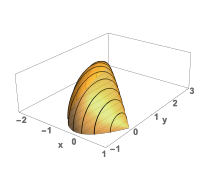
\includegraphics[scale=.5]{circ} % second figure itself
        \caption*{(c) Semicircles}
    \end{minipage}\hfill
\end{figure}

%%%%%%%%%%%%%%%%%%%%%%%%%%%%%%%%%%%%%%%%%%%%%%%%%%%%%%%%%%%%%%%%%%%%%%%%%%%%%%%%%%%%%%%%%%%% 8.1 WORK

\begin{enumerate}
\item First we need to find the area function, $A(x)$ of a cross section of the solid. We know that the height of the cross sectional shape is 2, therefore
\begin{align*}
A(x) &= 2\cdot S
\end{align*}
where $S$ is the length of the base. Notice that the lines of the base are parallel to the $y$-axis. Therefore,
\begin{align}
S &= (1-x)-(x^2-1)\\
&= 2-x-x^2
\end{align}
Thus our area function is 
\begin{align*}
A(x) &= 2(2-x-x^2)
\end{align*}
Next, we have to find the bounds of our integral which can be accomplished by finding the intersections between $y=1-x$ and $y=x^2-1$. Subtracting them gives the equation
\begin{align*}
0 &= 2-x-x^2\\
&= -\left(x^2+x-2\right)\\
&= -(x+2)(x-1)\\
&= (x+2)(x-1)
\end{align*}
Thus, we get the $x$-values for intersection as $x=1$, $x=-2$. Finally setting up the integral using the $x$-values as bounds, we get the integral
\[\int_{-2}^1\!\left(2x-2x^2\right)\,dx\]
\item The area function for a square is
\begin{align*}
A(x) &= S^2
\end{align*}
Using the our definition of $S$ from (1) and our bounds from part (a), we can set up the integral
\[\int_{-2}^1\!\left(2-x-x^2\right)^2\,dx\]
\item Using the same method as for the last two parts, we determine that the area function for this is 
\begin{align*}
A(x) &= \frac{\pi S^2}{2}
\end{align*}
Once more, we use the mathematics from part (a) to construct the integral
\[\int_{-2}^1\!\frac{\pi\left(2-x-x^2\right)^2}{2}\,dx\]
\end{enumerate}


\newpage
%%%%%%%%%%%%%%%%%%%%%%%%%%%%%%%%%%%%%%%%%%%%%%%%%%%%%%%%%%%%%%%%%%%%%%%%%%%%%%%%%%%%%%%%%%%% 8.2 PROBLEM

\item Let $S$ be the solid generated by rotating the region bounded by $y=x$ and $y=x^2$ around the line $y=-1$.
\begin{enumerate}
\item Sketch $S$
\item Use the method of washers to set up and evaluate an integral to find the value of $S$. Sketch a representative cross section on your drawing of $S$.
\end{enumerate}
%%%%%%%%%%%%%%%%%%%%%%%%%%%%%%%%%%%%%%%%%%%%%%%%%%%%%%%%%%%%%%%%%%%%%%%%%%%%%%%%%%%%%%%%%%%% 8.2 WORK

\begin{enumerate}
\item Figure Below
\begin{figure}[H]
\centering
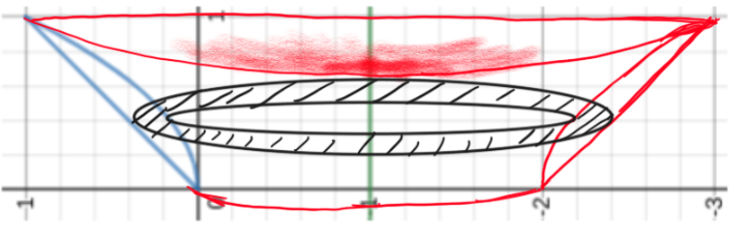
\includegraphics[scale=.5]{washer}
\end{figure}
\item We will use the general formula and find the variable values for them. The general equation is
\[\int_a^b\!\pi(f(x)^2-g(x)^2)\,dx\]
Since $S$ was rotated around the line $y=-1$ and not the $z$-axis, we must add one to our functions before writing them into the integrand. Letting $f(x)$ be the top function and $g(X)$ be the bottom, we can conclude  that
\begin{align*}
f(x) &= x+1\\
g(x) &= x^2+1\\
\end{align*}
The next step is to find the bounds of the integral. This is an relatively simple step, as all it requires is to find the intersection points of $y=x$ and $y=x^2$. Subtracting the two equations gives us
\begin{align*}
x^2-x &= 0\\
&= x(x-1)
\end{align*}
Giving us the bounds of $[a,b]$ as $[0,1]$. Thus we have our integral
\[\int_0^1\!\pi\left(\left(x+1\right)^2-\left(x^2+1\right)^2\right)\,dx\]
To compute this integral, first we must simplify which creates the simplified result of 
\[\pi\int_0^1\!-x^4-x^2+2x\,dx\]
Then, we use the Evaluation Theorem to evaluate the integral.
\begin{align*}
\pi\int_0^1\!-x^4-x^2+2x\,dx &= \pi\left[-\frac{x^5}{5}-\frac{x^3}{3}+x^2\right]_0^1\\
&= \pi\left(-\frac{1^5}{5}-\frac{1^3}{3}+1^2\right)-\pi\left(-\frac{0^5}{5}-\frac{0^3}{3}+0^2\right)\\
&= \pi\left(1-\frac{1}{3}-\frac{1}{5}\right)\\
&= \frac{7\pi}{15}
\end{align*}
Thus the volume of $S$ is $\dfrac{7\pi}{15}$.
\end{enumerate}

\newpage
%%%%%%%%%%%%%%%%%%%%%%%%%%%%%%%%%%%%%%%%%%%%%%%%%%%%%%%%%%%%%%%%%%%%%%%%%%%%%%%%%%%%%%%%%%%% 8.3 PROBLEM

\item Let $S$ be the solid generated by rotating the region bounded by $y=x$ and $y=x^2$ around the line $x=-1$.
\begin{enumerate}
\item Sketch $S$
\item Use the method of cylindrical shells to set up and evaluate an integral to find the value of $S$. Sketch a representative cross section on your drawing of $S$.
\end{enumerate}
%%%%%%%%%%%%%%%%%%%%%%%%%%%%%%%%%%%%%%%%%%%%%%%%%%%%%%%%%%%%%%%%%%%%%%%%%%%%%%%%%%%%%%%%%%%% 8.3 WORK

\begin{enumerate}

\item Figure Below
\begin{figure}[H]
\centering
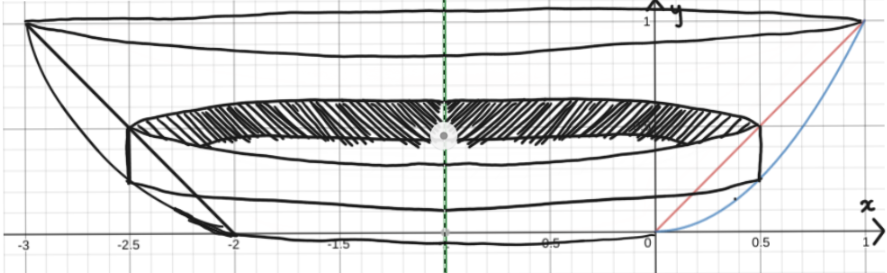
\includegraphics[scale=.5]{shell}
\end{figure}
\item To find the area of $S$, we need to use the integral,
\[\int_a^b\!2\pi xf(x)\,dx\]
We can find $f(x)$ by finding the vertical distance of the area bound by $y=x$ and $y=x^2$ which is $x-x^2$. Thus, our integral becomes
\[\int_a^b\!2\pi x(x-x^2)\,dx\]
Next, we replace $x$ with $1+x$, since the radius of the function will be one away from the $x$ of $f(x)$ since the solid is rotated around $x=-1$. Our bounds become $0$ and $1$ since the functions $y=x$ and $y=x^2$ intersect at $o$ and $1$. Thus, the final integral is
\[2\pi\int_0^1\!(1+x)(x-x^2)\,dx\]
The first step to evaluating this is to simplify. After simplification, the integral becomes
\[2\pi\int_0^1\!x-x^3\,dx\]
This becomes fairly simple to integrate, with the integration being
\begin{align*}
2\pi\int_0^1\!x-x^3\,dx &= 2\pi\left[\frac{x^2}{2}-\frac{x^4}{4}\right]_0^1\\
&= 2\pi\left(\frac{1^2}{2}-\frac{1^4}{4}\right)-2\pi\left(\frac{0^2}{2}-\frac{0^4}{4}\right)\\
&= 2\pi\left(\frac{1}{4}\right)\\
&= \frac{\pi}{2}
\end{align*}
The volume of $S$ is $\dfrac{\pi}{2}$.
\end{enumerate}

\newpage
%%%%%%%%%%%%%%%%%%%%%%%%%%%%%%%%%%%%%%%%%%%%%%%%%%%%%%%%%%%%%%%%%%%%%%%%%%%%%%%%%%%%%%%%%%%% 8.4 PROBLEM

\item \textbf{Professional Problem:}
\begin{enumerate}
\item Find the volume of the solid of revolution created by rotating the graph of $\sqrt{x}$, $0\le x\le9$, about the $x-$axis.
\item A different solid of revolution $S$ was created by rotating the same graph in part (a) around a line $y=k$ where $k>0$. The solid has the same volume as the solid in part (a). Find $k$.
\end{enumerate}
%%%%%%%%%%%%%%%%%%%%%%%%%%%%%%%%%%%%%%%%%%%%%%%%%%%%%%%%%%%%%%%%%%%%%%%%%%%%%%%%%%%%%%%%%%%% 8.4 WORK

\begin{enumerate}
\item We shall use the cylindrical shell method to find the volume of the solid of revolution created by rotating the graph of $\sqrt{x}$, $0\le x\le9$, about the $x-$axis. To do this, first we must find the area of one of these shells which is equal to the surface of a hollowed out cylinder. The surface area of a holow cylinder is $2\pi rh$ where $r$ is the radius and $h$ is the height. Since our cylinder lying down, $r=y$ and $h=9-x$, which means that if $y=\sqrt{x}$, then $h=9-y^2$. Thus, our shell surface area is 
\begin{align}
S(x) &= 2\pi y(9-y^2)
\end{align}
To find the volume we sum up and infinite number of the these cylinders from the $x$ values for which the function is defined. In this case, the integral from 0 to 3 of (3) since our function is in respect to $y$. Thus, the integral is
\begin{align*}
2\pi\int_0^3\!9y-y^3\,dy &= 2\pi\left[\frac{9y^2}{2}-\frac{y^4}{4}\right]_0^3\\
&= 2\pi\left(9\frac{3^2}{2}-\frac{3^4}{4}\right)\\
&= 2\pi(\frac{405}{4})\\
&= \frac{405\pi}{2}
\end{align*}
Thus, we have determined volume of the solid of revolution is $\dfrac{405\pi}{2}$.
\item To find $k$ we can define the integral
\[2\pi\int_0^3\!(k-y)(9-y^2)\,dy\]
is the volume of $S$. We convert $y$ to $k-y$ because the height is just the distance between $y=k$ and $y=\sqrt{x}$. Since we already know the volume of $S$, we can just plug it in and solve like so
\begin{align*}
\frac{405\pi}{2} &= 2\pi\int_0^3\!(k-y)(9-y^2)\,dy\\
\frac{405}{4} &= \int_0^3\!9k-ky^2+9y+y^3\,dy\\
&= \left[9ky-k\frac{y^3}{3}+9\frac{y^2}{2}+\frac{y^4}{4}\right]_0^3\\\\
&= 18k+\frac{243}{4}\\
\frac{162}{4} &= 18k\\
\frac{9}{4} &= k
\end{align*}
Using the evaluation theorem, we have found that $k=\dfrac{9}{4}$.
\end{enumerate}
%%%%%%%%%%%%%%%%%%%%%%%%%%%%%%%%%%%%%%%%%%%%%%%%%%%%%%%%%%%%%%%%%%%%%%%%%%%%%%%%%%%%%%%%%%%% END DOCUMENT


\end{enumerate}


\end{document}
